\documentclass[oneside]{homework} %%Change `twoside' to `oneside' if you are printing only on the one side of each sheet.
\usepackage{amsmath}
\usepackage{amssymb,mathtools}
\usepackage{graphicx}
\graphicspath{}

\studname{Alex Wong}
\studmail{asw2181@columbia.edu}
\coursename{COMS E6232}
\hwNo{2}
\uni{asw2181}

\begin{document}
\maketitle
\skipevenpage

\problemNo{1}
{\large a.} Consider an instance where we have two items x and y where $s_x = \epsilon$, $v_x = 2\epsilon$, $s_y = B$, $v_y =B$, and $\epsilon << 1$. The $v_i/s_i$ ratio of item x is 2 and item y is 1. Thus, the Greedy algorithm will always pick item x regardless of how large B is and regardless how small $\epsilon$ is. So as B gets larger and/or $\epsilon$ gets smaller, the approximation ratio of the algorithm will increase, thus showing that the approximation ratio of Greedy is not bounded by any constant. \hfill\qed
\newline
\newline
{\large b.} \textbf{Theorem 1b} The Modified Greedy algorithm achieves approximation ratio 2.
\newline

\textbf{Proof:} Let $OPT$ be the optimal solution that has maximum value where $v(OPT) = \sum\limits_{i\epsilon OPT}v_i$ subject to $\sum\limits_{i\epsilon OPT}s_i \leq B$. We first assume that the items are ordered in a non-increasing fashion according to the ratio $v_i/s_i$. Let's call the first item that does not fit in the knapsack using the Greedy algorithm as item $m$. We know that item $m$'s $v_i/s_i$ ratio $\geq$ items $m+1,...,n$'s $v_i/s_i$ ratio. Thus, if we are able to fit some fraction of item $m$ so that it fills up to the capacity of the knapsack, that solution will be $\geq$ OPT. We can define the fraction of item $m$ that fits into the knapsack as $\alpha$ where $\alpha = (B - \sum\limits_{i=1}^{m-1} v_i) / s_m$. Thus, $OPT \leq (\sum\limits_{i=1}^{m-1} v_i) + \alpha v_m$. Since $\alpha$ is some fraction $\leq 1$, we can also say that: $$OPT \leq (\sum\limits_{i=1}^{m-1} v_i) + \alpha v_m \leq (\sum\limits_{i=1}^{m-1} v_i) + v_m$$ From the inequality above, $\sum\limits_{i=1}^{m-1} v_i$ or $v_m$ must be at least $OPT/2$, showing that the Modified Greedy algorithm will always get a solution at least $OPT/2$, thus achieving an approximation ratio 2. \hfill\qed

\problemNo{2}
{\large a.} The lower bound for OPT is $max(max_i(p_i), \frac{\sum\limits_{i=1}^{n}p_i}{m})$. 
\newline
\newline
For $m$ = 2 machines and 5 jobs with processing times 3,3,2,2,2, the LPT algorithm will schedule 3,2,2 on $m_1$ and 3,2 on $m_2$, giving a makespan of 7. For OPT, we know that a lower bound is max = $max(3, 12/2) = 6$. We can achieve OPT by scheduling 2,2,2 on one machine and 3,3 on the other machine.
\newline
\newline
For $m$ = 3 machines and 7 jobs with processing times 5,5,4,4,3,3,3, the LPT algorithm will schedule 5,3,3 on $m_1$, 5,3 on $m_2$, and 4,4 on $m_3$, giving a makespan of 11. For OPT, the lower bound is $max(5, 27/3) = 9$. We can achieve OPT by scheduling 3,3,3 on one machine and 5,4 on each of the other two machines.
\newline
\newline
{\large b.} If $p_n > OPT/3$, then $3p_n > OPT$, showing that no machine can process more than 2 jobs or else it would be $>$ OPT, which would contradict OPT being the optimal solution. From this, we know that $n \leq 2m$, thus the largest $m$ jobs will first get scheduled on each of the $m$ machines and the rest of the $n - m$ jobs will be assigned to the machine that has the least load at the point of assignment, thus showing that the LPT schedule is optimal. \hfill\qed
\newline
\newline
{\large c.} \textbf{Theorem 2c} LPT achieves an approximation ratio of 4/3.
\newline

\textbf{Proof:} Let's define job $j$ as the job that finishes last in the LPT schedule and $t_j$ as the span of time from time 0 until the time that job $j$ starts. We know that in the timespan of $t_j$, $m\cdot t_j$ amount of processing has been done. This amount of processing can't be more than the total amount of processing of all jobs, thus $m \cdot t_j \leq \sum\limits_{i=1}^{n}p_i \implies t_j \leq \frac{\sum\limits_{i=1}^{n}p_i}{m}$. As we saw earlier in part $a$, $\frac{\sum\limits_{i=1}^{n}p_i}{m}$ is essentially a lower bound for OPT, thus we can say that $t_j \leq OPT$. Then by adding $p_j$ to $t_j$, we get the makespan of the machine that has scheduled job $j$, and we can say that $t_j + p_j \leq OPT + p_j$. What the inequality tells us is that the processing time of job $j$ indicates how well the LPT algorithm performs. Referring to part $b$, if $p_j > OPT/3$, the LPT schedule is optimal. But in the worst case, if $p_j = OPT/3$, then LPT will give an $OPT + p_j = OPT + OPT/3 = 4/3 OPT$ makespan, thus showing that LPT achieves an approximation ratio of 4/3. \hfill\qed
\newline
\newline
{\large d.} \textbf{Theorem 2d} The ratio of 4/3 of LPT is asymptotically tight as $m \rightarrow \infty$.
\newline

\textbf{Proof:} We generalize the examples of part $a$: given $m$ machines, we have 3 jobs that have a processing time of $m$, and 2 jobs for each processing time $2m-1,...,m+1$ (if $2m-1 = m+1$, then there are only 2 jobs for both $2m-1$ and $m+1$) giving us a total of 2m+1 jobs. With LPT scheduling, we find that every machine will get scheduled two jobs with a total processing time of $3m-1$ with exception of the first machine that will get scheduled with 3 jobs with a total processing time of $3m-1+m = 4m-1$. Thus, the makespan with LPT scheduling is $4m-1$. For an optimal makespan $OPT$, we first schedule all 3 jobs with processing time $m$ on the first machine, and then use LPT scheduling for the rest of the jobs. This will give each machine a total processing time of $3m$, thus making the makespan of $OPT = 3m$. Without loss of generality, the figure below illustrates the makespan of LPT and $OPT$ of the example from part $a$ when $m = 3$:
\begin{figure}[h]
\centering
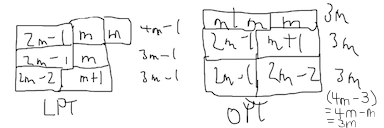
\includegraphics{2d1}
\caption{Makespan of LPT = 4m - 1, Makespan of OPT = 3m}
\end{figure}
\newline
Thus, we see the ratio of $LPT/OPT = (4m - 1) / 3m = \frac{4m}{3m} - \frac{1}{3m} = \frac{4}{3} - \frac{1}{3m}$, showing that the approximation ratio 4/3 is asymptotically tight as $m \rightarrow \infty$. \hfill\qed

\problemNo{3}
{\large a.} \textbf{Proof:} An optimal schedule will have all on-time jobs complete before all late jobs because the objective is to schedule jobs to maximize the total weight of the jobs that complete by their due date; any late jobs' weight will not count towards the total weight,  essentially having a weight of 0 in the optimal schedule since they are late. We can also equally reframe the objective of maximizing weight of on-time jobs to minimizing weight of late jobs. By ordering jobs in an earliest due date order, we can achieve minimizing weight of late jobs, which means maximizing the total weight of on-time jobs, thus showing that an optimal schedule has all on-time jobs complete before late jobs and on-time jobs complete in an earliest due date order. \hfill\qed
\newline
\newline
{\large b.} There are $n$ jobs where job $j$ has processing time $p_j$, a weight $w_j$, and a due date $d_j$, where $j = 1,...,n$. Let $W = \sum\limits_{j}w_j$ which signifies the maximum possible value an optimal schedule can achieve, where every job completes on time. We use the following Dynamic Programming algorithm to compute the optimal schedule with a maximum total weight of jobs that complete by their due date:
\newline
\newline
\textbf{DP Scheduling Algorithm}
\newline
\newline
\textbf{Preprocessing:} We first order the jobs by nondecreasing due date order, which takes $O(nlogn)$ time, where n is the number of jobs to be scheduled. It will not affect the overall runtime since the overall runtime of the algorithm is $O(nW)$ where $W$ has a lower bound of $n$ since each job has weight is a positive integer, making $O(nW) \geq O(n^2)$, which is $>$ $O(nlogn)$.
\newline
\newline
\textbf{DP Initialization:} Let A be a table that stores values of minimum completion times. Let $A(w, j)$ represent the minimum completion time of a subset of jobs $1,...,j$ that are on-time and adding all on-time jobs' weights gives the total weight of $w$. If there is no feasible subset, then $A(w,j) = \infty$. We initalize $A(0,j) = 0$, for all $j = 0,...,n$ because to get a total weight of 0, we do not need to have any on-time jobs, thus having a minimum completion time of 0. We initialize $A(w,0) = \infty$, for all $w = 1,...,W$ where $W = \sum\limits_{j}w_j$ because it is not feasible to get some total weight $> 0$ without having a subset of jobs to schedule. Because we are doing constant work on $n + W$ entries of table A, DP initialization has a runtime of $O(n + W)$.
\newline
\newline
\textbf{DP Recursion:} 
\newline
For $1 \leq w \leq W, \ 1 \leq j \leq n$, if job $j$ is not an on-time job, we know then that the subset of jobs $1,...,j-1$ offers the minimum completion time at that weight w. If job $j$ is an on-time job, as in $A(w-w_j, j-1) + p_j \leq d_j$, then we take the minimum completion time between the minimum completion time of subset of jobs $1,...,j-1$ at weight w or the minimum completion time of subset of jobs $1,...,j-1$ at weight $w-w_j$ since jobs $1,...,j-1$ will have at least $w-w_j$ weight, added with the processing time $p_j$ of job $j$. The following equation shows the recursion:
\newline
\newline
For $1 \leq w \leq W, \ \ 1 \leq j \leq n$:
\begin{equation*}
  A(w,j) =
  \begin{cases}
    min(A(w, j-1), A(w-w_j, j-1) + p_j) & \text{if $w \geq w_j$ and $A(w-w_j, j-1) + p_j \leq d_j$} \\
    A(w, j-1) & \text{otherwise}
  \end{cases}
\end{equation*}
For the runtime of DP recursion, we see that we do a constant amount of work for $n\cdot W$ entries of table $A$, thus the runtime of DP recursion is $O(nW)$.
\newline
\newline
\textbf{DP Answer:}
\newline
Let OPT be the maximum total weight of jobs that complete by their due date. After filling out table A, the maximum weight of on-time jobs is: $$OPT = max\{ w \ | \ A(w,n) \neq \infty \}$$ which takes $O(W)$ running time. Thus, the total running time is $$O(nlogn) + O(n + W) + O(nW) + O(W) = O(nW)$$ \hfill\qed
\newline
\newline
{\large c.} \textbf{FPTAS for Scheduling Problem:}
\begin{itemize}
  \item Lets first define $W' = max_j (w_j),$ where $j = 1,...,n$.
  \item Since $W = \sum\limits_{j=1}^{n}w_j$, we can say that $W \leq nW'$.
  \item Assume, without loss of generality, that $\epsilon \leq 1$.
  \item Let $K = \epsilon W' / 2n$.
  \item Now, for each job $j$, let $w'_j = \lfloor\frac{w_j}{K}\rfloor$
  \item Then $W'' = max_j(w'_j) ,= \lfloor\frac{W'}{K}\rfloor = \lfloor\frac{W'}{\epsilon W'/2n}\rfloor = \lfloor\frac{2n}{\epsilon}\rfloor$
\end{itemize}
\textbf{Runtime:} 
\newline
Applying the DP algorithm from part $b$ with these new weights $w'_j$ and a new total max weight of $nW''$, with everything else remaining the same, we get a runtime of $O(n\cdot(nW'')) = O(n\cdot(n\cdot\frac{2n}{\epsilon})) = O(n^3/\epsilon)$ which is a runtime that is both polynomial in $n$ and $1/\epsilon$.
\newline
\newline
\textbf{Approximation Ratio:} 
\newline
Let's define $Q$ as an optimal solution using the original weights and $S$ as an optimal solution using the new weights $w'_j$.
\newline
For each job $j$, we know that: $\frac{w_j}{K} - 1 < w'_j \leq \frac{w_j}{K}$. This implies that: 
$$\frac{\sum\limits_{j\epsilon S}w_j}{K} - |S| < \sum\limits_{j\epsilon S}w'_j \leq \frac{\sum\limits_{j\epsilon S}w_j}{K}$$
For OPT, we know that: 
$$OPT = w(Q) = \sum\limits_{j\epsilon Q}w_j \ \text{which tells us} \ \frac{w(Q)}{K} - |Q| < w'(Q) \leq w'(S)$$ 
$$\Longrightarrow \ w(Q) \leq K \cdot w'(S) + K \cdot |Q| \leq w(S) + K \cdot n$$
$$\Longrightarrow \ w(Q) \leq w(S) + \frac{\epsilon}{2}W' \leq w(S) + \frac{\epsilon}{2}w(Q), \ \text{because} \ W' \leq w(Q)$$
From here, we can say that:
$$w(Q) \leq w(S) + \frac{\epsilon}{2}w(Q)$$
$$\Longrightarrow w(Q) - \frac{\epsilon}{2}w(Q) \leq w(S)$$
$$\Longrightarrow w(Q) \cdot (1 - \frac{\epsilon}{2}) \leq w(S)$$
And since we are looking for the approximation ratio:
$$\frac{OPT}{w(S)} = \frac{w(Q)}{w(S)} \leq \frac{w(Q)}{w(Q) \cdot (1 - \frac{\epsilon}{2})} = \frac{1}{1 - \frac{\epsilon}{2}} \leq 1 + \epsilon, \ \text{since} \ \ \epsilon \leq 1$$
Thus showing that the approximation ratio is $1 + \epsilon$.
\newline
\newline
\textbf{Conclusion:} We have provided a FPTAS for the Scheduling problem by scaling and rounding the weights of each job, which resulted in a runtime polynomial in both $n$ and $1/\epsilon$ with an approximation ratio of $1 + \epsilon$.\hfill\qed

\problemNo{4}
{\large a.} To get a pseudopolynomial algorithm for the Assembly problem, we utilize dynamic programming.
\newline
\newline
\textbf{DP Assembly Algorithm}
\newline
\newline
\textbf{Preprocessing:} We first define $n$ as the number of all choices of all components, which equates to $\sum\limits_{i=1}^{k}|S(i)|$. We then define a max cost $C$ for our DP algorithm to run on by summing up the max cost of a choice from each set $S(i)$ choices where $i = 1,...,k$ . Thus, $C = \sum\limits_{i=1}^{k}max_x(S(i)_x)$ for $x = 1,...,|S(i)|$. This takes $O(n)$ runtime since we have to iterate through all choices of all components, which we have defined as $n$.
\newline
\newline
\textbf{DP Initialization:} Let A be a table that stores values of minimum weights. Let $A(c, i)$ represent the minimum weight of a subset of components $1,...,i$ that have a weight below $W$ and adding all subset of components' costs gives the total cost of $c$. If there is no feasible subset, then $A(c,i) = \infty$. We first initialize $A(0,0) = 0$ because having 0 components with 0 costs means a 0 weight. We then initialize $A(0,i) = \infty$, for all $i = 1,...,k$ because to we can not get a total cost of 0 for any number of components $> 0$ since costs are positive integers. We initialize $A(c,0) = \infty$, for all $c = 1,...,C$ because it is not feasible to get some total cost $> 0$ without having some subset of components to work with. Because we are doing constant work on $k + C$ entries of table A, and $k \leq n$ since each set of choices $S(i)$ must contain at least one choice, DP initialization has a runtime of $O(n + C)$.
\newline
\newline
\textbf{DP Recursion:} 
\newline
For $1 \leq c \leq C, \ 1 \leq i \leq k$, we iterate through the set of choices $S(i)$, where each choice will be denoted $S(i)_x$, $x = 1,...,|S(i)|$, to find the minimum weight choice that doesn't exceed the upper bound weight W when the weight $w_{S(i)_x}$ is added to the subset of components $1,...i-1$ and where the cost of the subset of components $1...,i-1$ has cost $c - c_{S(i)_x}$ so that if choice $S(i)_x$ is included, the cost will equal $c$. The last constraint is that $A(c-c_{S(i)_x}, i-1) \neq \infty$ because that signifies that there wasn't a feasible subset from components $1,...i-1$ so there is no point to add component $S(i)_x$ since there wasn't any feasible subset before. If no choice $S(i)_x$ meets the constraints, then $A(c,i) = \infty$. The following equation shows the recursion:
\newline
\newline
For $1 \leq c \leq C, \ \ 1 \leq i \leq k$:
\begin{equation*}
  A(c,i) = min
  \begin{cases}
    A(c-c_{S(i)_1}, i-1) + w_{S(i)_1} & \text{if $c \geq c_{S(i)_1}$,} \\
    . & \text{$A(c-c_{S(i)_1}, i-1) \neq \infty$ ,} \\
    . & \text{and $A(c-c_{S(i)_1}, i-1) + w_{S(i)_1} \leq W$} \\
    . \\
    . \\
    A(c-c_{S(i)_{|S(i)|}}, i-1) + w_{S(i)_{|S(i)|}} & \text{if $c \geq c_{S(i)_{|S(i)|}}$,} \\
     & \text{$A(c-c_{S(i)_{|S(i)|}}, i-1) \neq \infty$} \\
     & \text{and $A(c-c_{S(i)_{|S(i)|}}, i-1) + w_{S(i)_{|S(i)|}} \leq W$} \\
     \\
    \infty & \text{otherwise}
  \end{cases}
\end{equation*}
\newline
For the runtime of DP recursion, we see that we do $\sum\limits_{i=1}^{k}|S(i)| = n$ amount of work for $C$ number of rows of table $A$, thus the runtime of DP recursion is $O(nC)$.
\newline
\newline 
\textbf{DP Answer:}
\newline
Let OPT be the minimum cost to assemble a product that meets the upper bound weight W. After filling out table A, the minimum cost to assemble a product is: $$OPT = min\{ c \ | \ A(c,i) \}$$ If we find that $OPT = \infty$, then that means there was no combination of components that could make a product with a weight $\leq W$. The running time to find OPT takes $O(C)$. Thus, the total running time is $$O(n) + O(n + C) + O(nC) + O(C) = O(nC)$$ which shows that the DP algorithm is a pseudopolynomial algorithm for the Assembly problem. \hfill\qed
\newline
\newline
{\large b.} \textbf{FPTAS for Assembly Problem:}
\begin{itemize}
  \item Lets first define $C'$ as the maximum cost of any choice of any component $S(i)_x$, where $i = 1,...,k$ and $x = 1,...,|S(i)|$. Thus $C' = max_i(max_x(c_{S(i)_x}))$.
  \item Since $C = \sum\limits_{i=1}^{k}max_x(c_{S(i)_x})$ for $x = 1,...,|S(i)|$, we can say that $C \leq kC'$.
  \item Assume, without loss of generality, that $\epsilon \leq 1$.
  \item Let $K = \epsilon C' / 2k$.
  \item Now, for each choice $S(i)_x$, let $c'_{S(i)_x} = \lceil\frac{c_{S(i)_x}}{K}\rceil$
  \item Then $C'' = max_i(max_x(c'_{S(i)_x})) ,= \lceil\frac{C'}{K}\rceil = \lceil\frac{C'}{\epsilon C'/2k}\rceil = \lceil\frac{2k}{\epsilon}\rceil$
\end{itemize}
\textbf{Runtime:} 
\newline
Applying the DP algorithm from part $a$ with these new costs $c'_{S(i)_x}$ and a new total max cost of $nC''$, with everything else remaining the same, we get a runtime of $$O(n\cdot(kC'')) = O(n\cdot(k\cdot\frac{2k}{\epsilon})) \leq O(n\cdot(n\cdot\frac{2n}{\epsilon})) = O(n^3/\epsilon)$$ ($k \leq n$ since each set of choices $S(i)$ must contain at least one choice) which is a runtime that is both polynomial in $n$ and $1/\epsilon$.
\newline
\newline
\textbf{Approximation Ratio:} 
\newline
Let's define $Q$ as an optimal solution using the original costs $c_{S(i)_x}$ and $R$ as an optimal solution using the new costs $c'_{S(i)_x}$.
\newline
For each choice $S(i)_x$, we know that: $\frac{c_{S(i)_x}}{K} + 1 > c'_{S(i)_x} \geq \frac{c_{S(i)_x}}{K}$. This implies that: 
$$\frac{\sum\limits_{S(i)_x\epsilon R}c_{S(i)_x}}{K} + |R| > \sum\limits_{S(i)_x\epsilon R}c'_{S(i)_x} \geq \frac{\sum\limits_{S(i)_x\epsilon R}c_{S(i)_x}}{K}$$
For OPT, we know that: 
$$OPT = c(Q) = \sum\limits_{S(i)_x\epsilon Q}c_{S(i)_x} \ \text{which tells us} \ \frac{c(Q)}{K} + |Q| > c'(Q) \geq c'(R)$$ 
$$\Longrightarrow \ c(Q) \geq K \cdot c'(R) - K \cdot |Q| \geq c(R) - K \cdot k$$
$$\Longrightarrow \ c(Q) \geq c(R) - \frac{\epsilon}{2}C' \geq c(R) - \frac{\epsilon}{2}\cdot\frac{c(Q)}{|Q|} = c(R) - \frac{\epsilon}{2}\cdot\frac{c(Q)}{k}, \ \text{because} \ C' \geq \frac{c(Q)}{k}$$
From here, we can say that:
$$c(Q) \geq c(R) - \frac{\epsilon}{2}\cdot \frac{c(Q)}{k}$$
$$\Longrightarrow c(R) \leq c(Q) + \frac{\epsilon}{2k}c(Q)$$
$$\Longrightarrow c(R) \leq c(Q) \cdot (1 + \frac{\epsilon}{2k})$$
And since we are looking for the approximation ratio:
$$\frac{OPT}{c(R)} = \frac{c(Q)}{c(R)} \geq \frac{c(Q)}{c(Q) \cdot (1 + \frac{\epsilon}{2k})} = \frac{1}{1 +\frac{\epsilon}{2k}} \geq 1 - \epsilon, \ \text{since} \ \ \epsilon \leq 1 \ \text{and} \ k \geq 1$$
\newline
Thus showing that the approximation ratio is $1 - \epsilon$.
\newline
\newline
\textbf{Conclusion:} We have provided a FPTAS for the Assembly problem by scaling and rounding the weights of each choice, which resulted in a runtime polynomial in both $n$ and $1/\epsilon$ with an approximation ratio of $1 - \epsilon$.\hfill\qed
\end{document}